% CREATED BY DAVID FRISK, 2016
\section{Results}
The results from both the pre-evolution process and the main simulation are presented in this Section. When possible, figures have been used to more clearly represent the data. In the case of the movement of the robot, care has been taken to describe the dynamics as accurately as possible.

\subsection{Processed data}
The processed data was plotted in a graph to identify walking cycles, see Appendix \ref{ProcessedData}. As this plot contained too much information to give a clear image and for clarity, two plots were made containing only the information from the left and right hip's acceleration in the z-axis which was enough to check for a pattern. These plots can be viewed in Figure \ref{fig:WalkingCycles}, where walking cycles can be clearly identified.


\begin{figure}[H]
    \centering
    \begin{subfigure}[b]{0.5\textwidth}
        \centering
        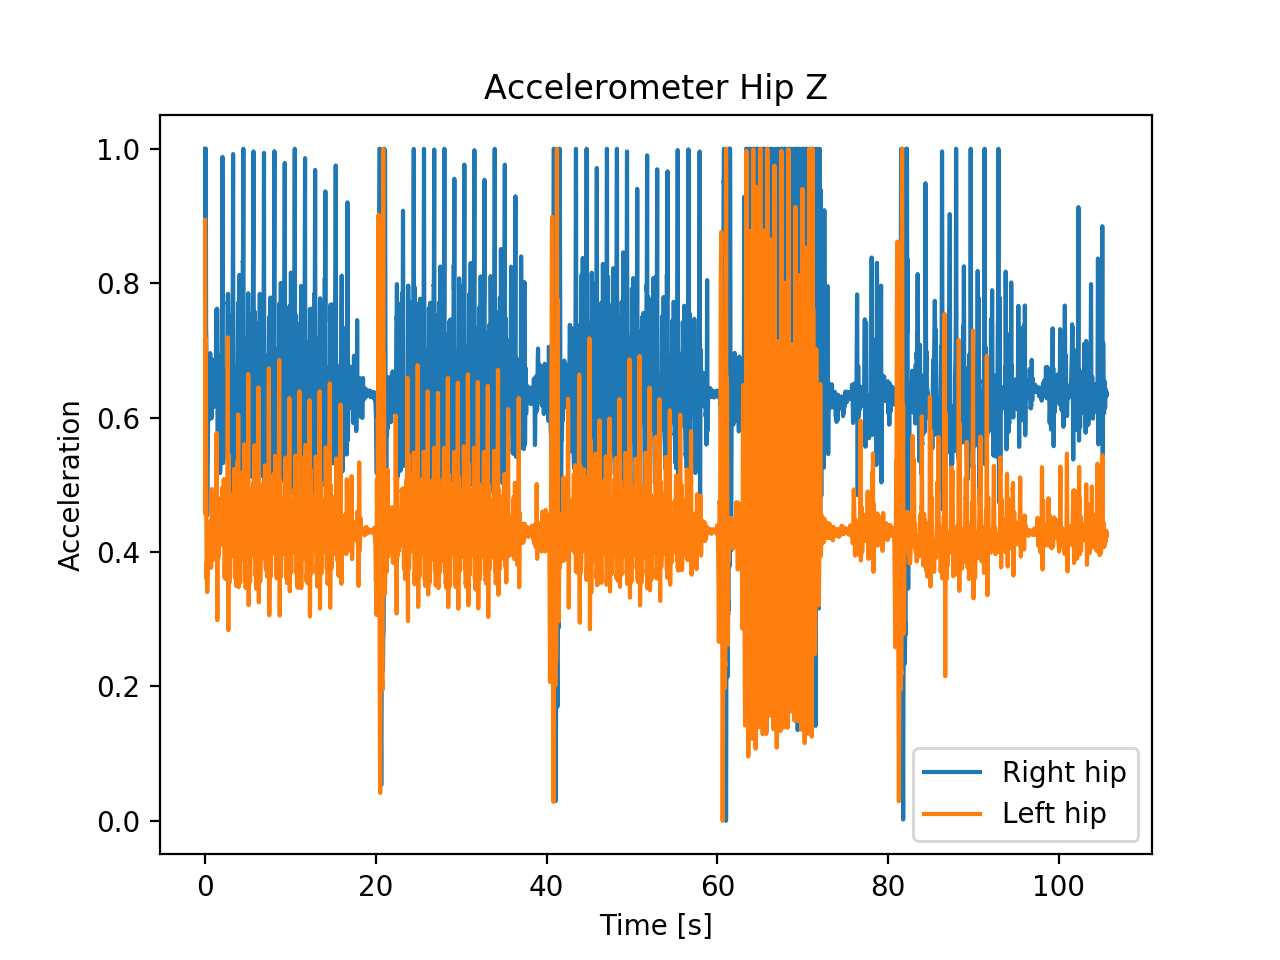
\includegraphics[width=1\textwidth]{include/figure/RLH5.png}
        \caption{Plot of the gathered data from five walking cycles.}
        \label{fig:RLH5}
    \end{subfigure}%
    ~ 
    \begin{subfigure}[b]{0.5\textwidth}
        \centering
        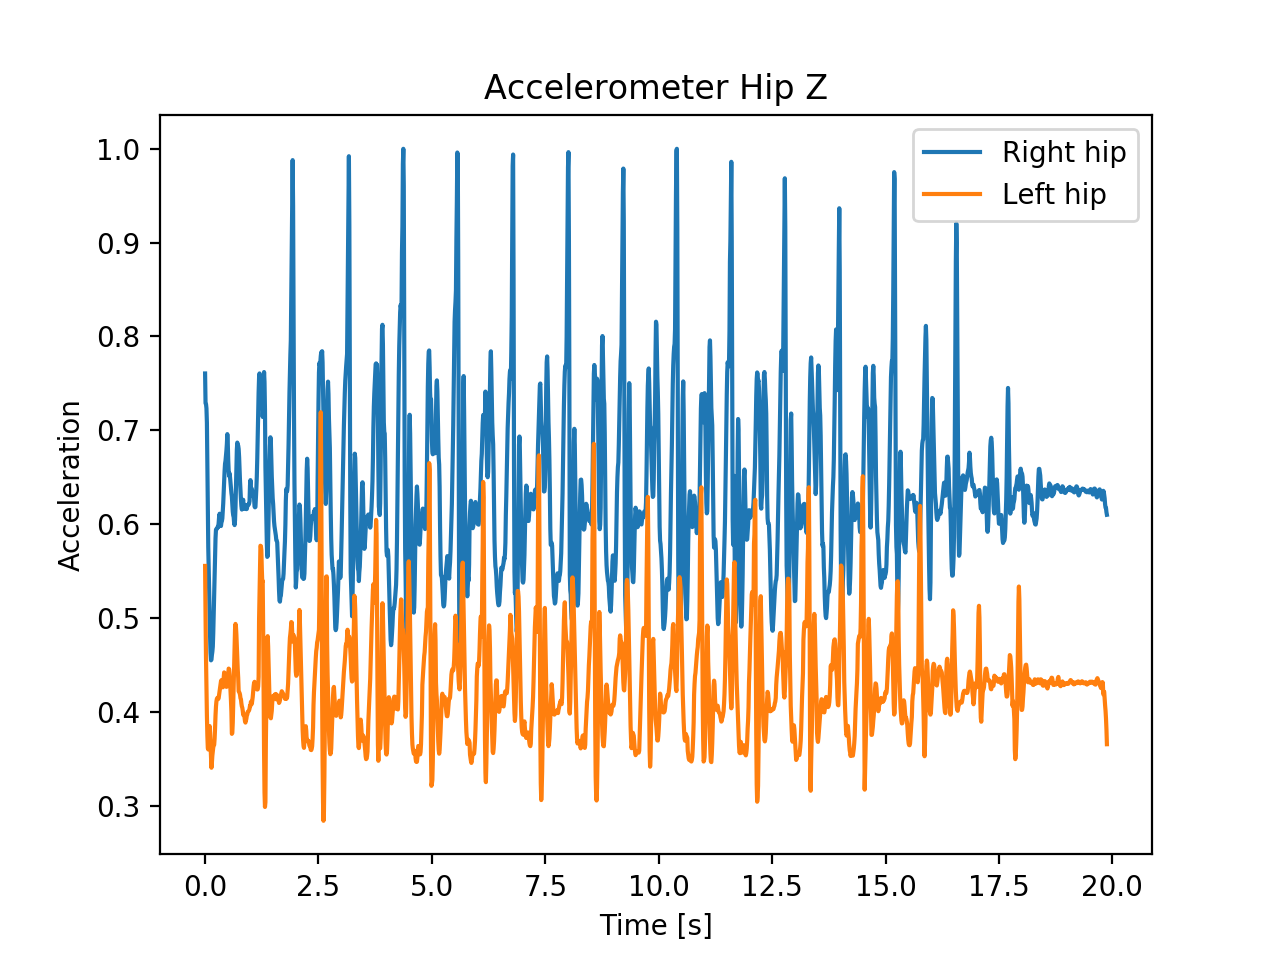
\includegraphics[width=1\textwidth]{include/figure/RLH1.png}
        \caption{Plot of the gathered data from one walking cycle.}
        \label{fig:RLH1}
    \end{subfigure}
    \caption{Processed Data from the recorded walking cycles.}
    \label{fig:WalkingCycles}
\end{figure}

\subsection{Pre-Evolution}
Simulation of the CPG model was done over 20 seconds with a timestep of 0.01 seconds, corresponding to the time of one recorded walking cycle. The population size varied between 20-40 individuals depending on simulations. Full-scale evolutions were made with 500-1000 generations.

\begin{figure*}[htbp]
    \centering
        
    \begin{subfigure}[b]{0.45\textwidth}
        \centering
        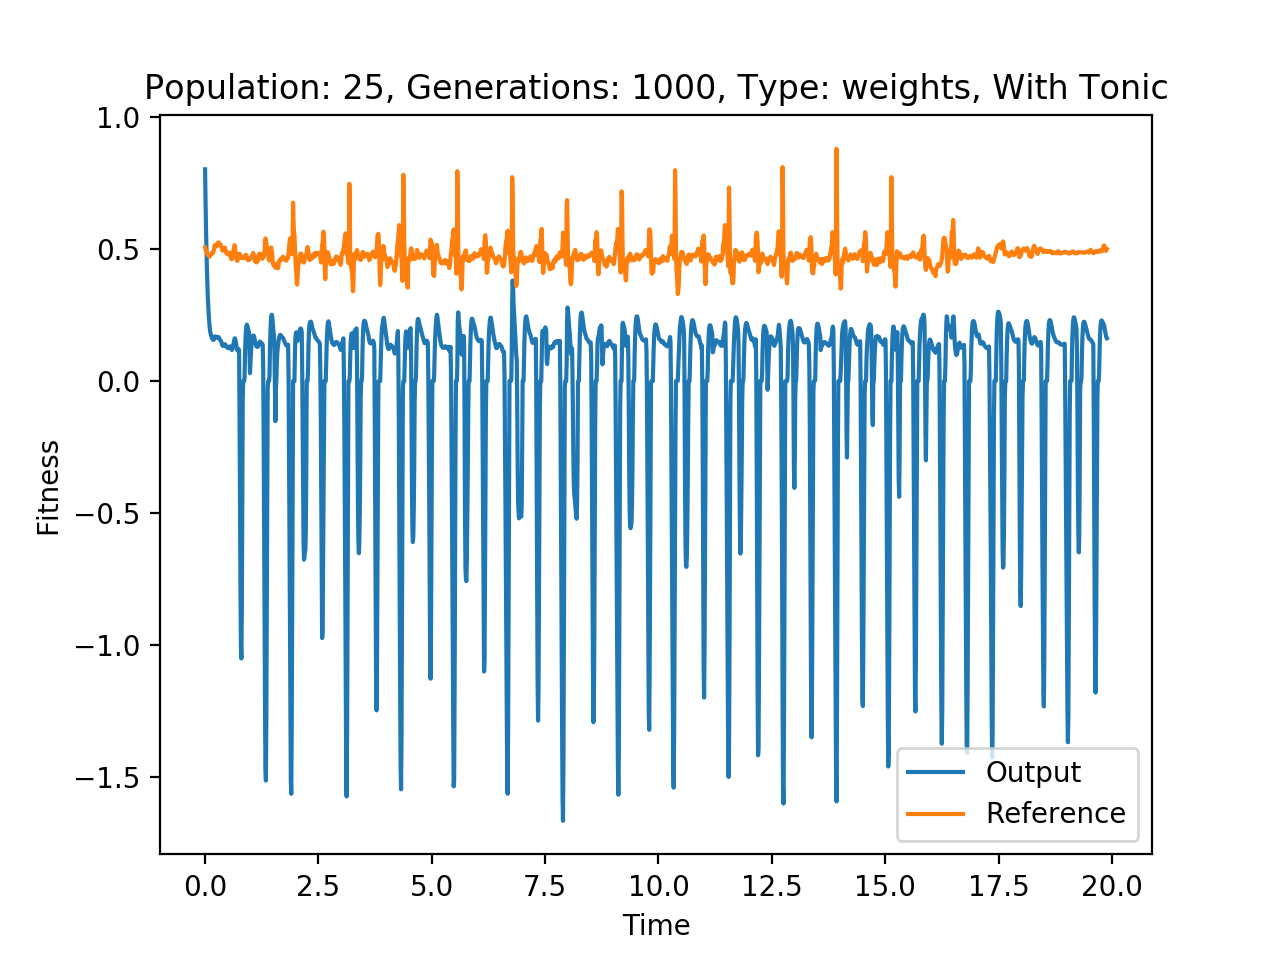
\includegraphics[width=0.95\textwidth]{include/figure/output_pop25_gen1000_type0_with.png}
        \caption{Original version.}
        \label{fig:result_1a}
    \end{subfigure}
    ~ 
    \begin{subfigure}[b]{0.45\textwidth}
        \centering
        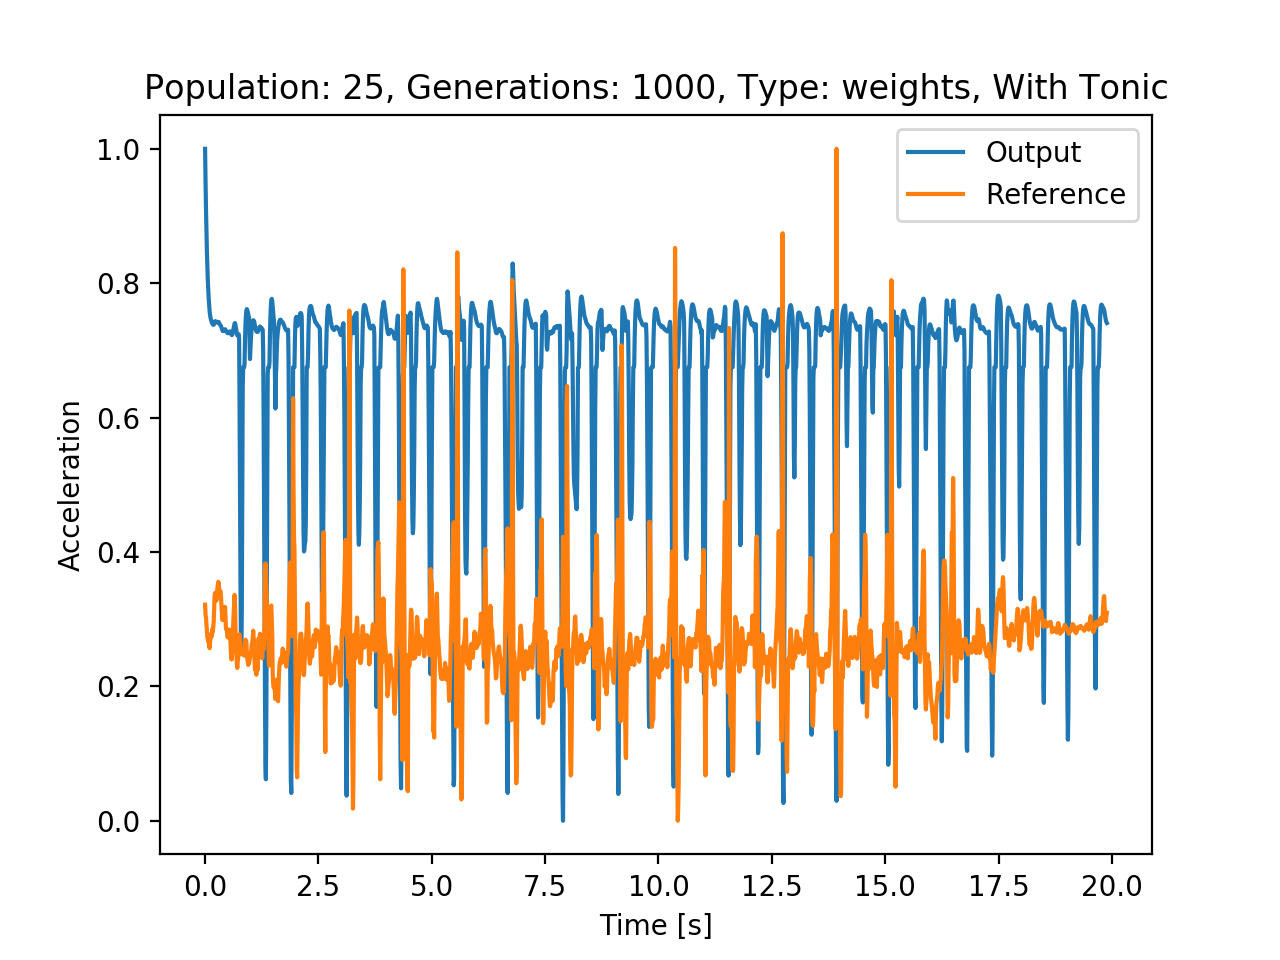
\includegraphics[width=0.95\textwidth]{include/figure/best_individual_output_pop25_gen1000_type0_with_normalised.png}
        \caption{Normalised version.}
        \label{fig:result_1b}
    \end{subfigure}%
    \caption{Output signals of the CPG network.}
    \label{fig:result_1}
\end{figure*}

As seen in Figure \ref{fig:result_1a}, the amplitude of the output signal does not match the amplitude of the reference signal. To easier compare the signals, the output signals were normalised, which can be seen in Figure \ref{fig:result_1b}. It can be seen that the pre-evolution simulation manage to create rhytmic output patterns, but does not manage to match the amplitude of the reference signals significantly. This is confirmed by the fitness scores, shown in Figure \ref{fig:fitness_1}. The fitness is maximally around 4\% correlation, which is quite low, since they ideally should be fully correlated. When using the entire Bioloid as type, it refers to using both the internal parameters in the CPG as well as the weights between them as genome. Further results are shown in Appendix \ref{resultsOfPreEvolution}.

\begin{figure*}[htbp]
    \centering
    \begin{subfigure}[b]{0.5\textwidth}
        \centering
        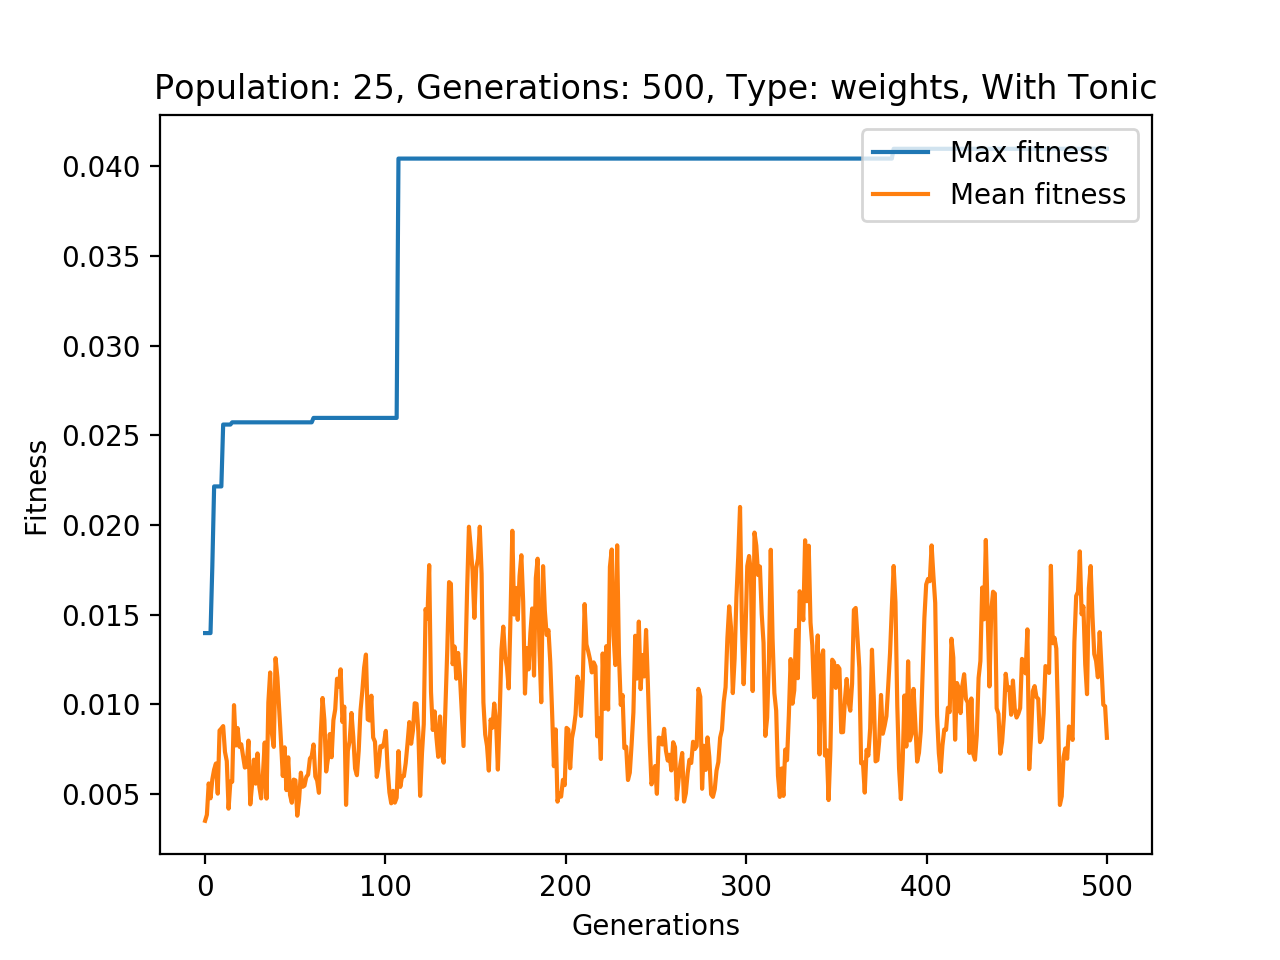
\includegraphics[width=1\textwidth]{include/figure/fitness_over_time_pop25_gen500_type0_with.png}
        \caption{Only weights. \vspace{0.5cm}}
        \label{fig:fitness_1a}
    \end{subfigure}%
    ~ 
    \begin{subfigure}[b]{0.5\textwidth}
        \centering
        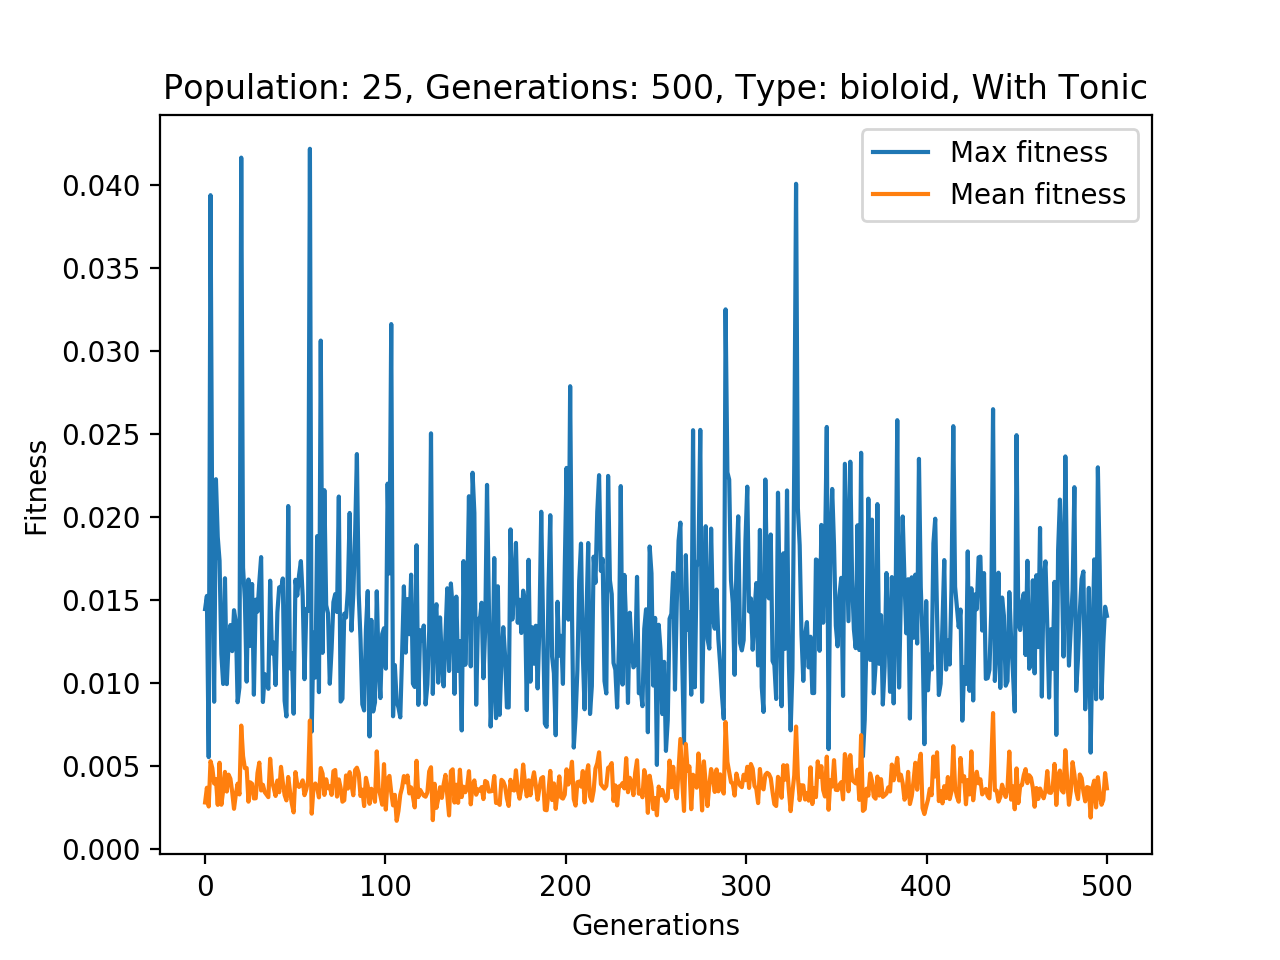
\includegraphics[width=1\textwidth]{include/figure/fitness_over_time_pop25_gen500_type1_with.png}
        \caption{Entire bioloid, both weights and internal parameters.}
        \label{fig:fitness_1b}
    \end{subfigure}
    \caption{The evolution of the fitness function.}
    \label{fig:fitness_1}
\end{figure*}


\subsection{Simulation}
In the case of the 18 DoF simulation with the support rods attached to the Bioloid robot, the Bioloid never achieved a walking cycle. From the start, the simulation with four rods did not properly converge into a stable cycle, which propagated to the case with two support rods, and further in the simulation with no support rods. The initial values were evidently too unstable for the robot to support itself, even if it did display some rudimentary capability to throw itself forward rather than backward. With these results, efforts were focused on the simulations where the external support arm was present, both with 8 and 18 degrees of freedom. Here the results are more closely overlapping, but as expected the 18 DoF simulation is more unstable than the 8 DoF simulation. 

Neither simulation achieves a walking cycle comparable to the data gathered from the accelerometers, which means it is quite far off from a humanoid walking cycle. Both movement cycles seem to mainly exploit the fact that in the simulation, it is possible to inch the robot forward by extending one leg and wobbling the foot servo, generating a small amount of friction that slowly pulls the robot forward. However, this does not hold up when applied to the physical Bioloid, since the friction coefficient is completely different, caused by the reality gap. This can probably be tweaked by changing the friction material (modeling clay in this case) to something with less grip, possibly allowing the Bioloid to inch forward like in the simulation.